\section{结果与对比}
\label{sec:results}

\subsection{端部与中截面位移}

Q4 与 CST 在 $160\times32$ 网格上均已高度接近 CalculiX 参考；一维杆只在 A 级工况可信。五种工况的端/中截面平均位移见 表~\ref{tab:disp-end} 与 表~\ref{tab:disp-mid}，相对 CCX 参考的偏差见 表~\ref{tab:dev}。Q4 的端/中位移最大偏差为 $0.025\%/0.014\%$，CST 为 $0.075\%/0.067\%$。相对一维解，S0、S1、S2 的偏差在 $0.6\%$ 以内；S3 端部偏差约 $3.3\%$，S4 约 $7.9\%$，已超出工程可接受范围。

\begin{table}[htbp]
  \centering
  \caption{端截面平均位移 $u_{\rm end}$（$\si{\micro\metre}$，$160\times32$ 网格）。}
  \label{tab:disp-end}
  \small
  \begin{tabular}{@{}lS[table-format=1.6]S[table-format=1.6]S[table-format=1.6]S[table-format=1.6]S[table-format=1.6]@{}}
\toprule
工况 & {1D} & {杆} & {Q4} & {CST} & {CCX CPS8} \\
\midrule
S0 & 0.250000 & 0.250000 & 0.249379 & 0.249368 & 0.249380 \\
S1 & 0.173287 & 0.173287 & 0.174238 & 0.174220 & 0.174238 \\
S2 & 0.346574 & 0.346574 & 0.346400 & 0.346390 & 0.346395 \\
S3 & 0.086643 & 0.086643 & 0.089506 & 0.089480 & 0.089520 \\
S4 & 0.091551 & 0.091551 & 0.098794 & 0.098745 & 0.098819 \\
\bottomrule
\end{tabular}

\end{table}

\begin{table}[htbp]
  \centering
  \caption{中截面平均位移 $u_{\rm mid}$（$\si{\micro\metre}$，$160\times32$ 网格）。}
  \label{tab:disp-mid}
  \small
  \begin{tabular}{@{}lS[table-format=1.6]S[table-format=1.6]S[table-format=1.6]S[table-format=1.6]S[table-format=1.6]@{}}
\toprule
工况 & {1D} & {杆} & {Q4} & {CST} & {CCX CPS8} \\
\midrule
S0 & 0.125000 & 0.125000 & 0.124379 & 0.124368 & 0.124380 \\
S1 & 0.101366 & 0.101366 & 0.101423 & 0.101406 & 0.101420 \\
S2 & 0.143841 & 0.143841 & 0.143423 & 0.143413 & 0.143429 \\
S3 & 0.050683 & 0.050683 & 0.051273 & 0.051253 & 0.051280 \\
S4 & 0.057762 & 0.057762 & 0.060221 & 0.060189 & 0.060229 \\
\bottomrule
\end{tabular}

\end{table}

\begin{table}[htbp]
  \centering
  \caption{相对 CalculiX CPS8 $240\times48$ 参考的偏差（$160\times32$，单位：\%）。$e_{\rm end}$、$e_{\rm mid}$ 为位移偏差，$e_\sigma$ 为探针点应力偏差。一维杆的偏差定义为 $(u_{\rm bar}-u_{\rm ref})/u_{\rm ref}$。}
  \label{tab:dev}
  \footnotesize
  \setlength{\tabcolsep}{4pt}
  \begin{tabular}{@{}lS[table-format=+1.2]S[table-format=+1.4]S[table-format=+1.4]S[table-format=+1.4]S[table-format=+1.4]S[table-format=1.4]S[table-format=1.4]@{}}
\toprule
工况 & {杆 $e_{\rm end}$} & {Q4 $e_{\rm end}$} & {Q4 $e_{\rm mid}$} & {CST $e_{\rm end}$} & {CST $e_{\rm mid}$} & {Q4 $e_\sigma$} & {CST $e_\sigma$} \\
\midrule
S0 & +0.249 & -0.0002 & -0.0004 & -0.0047 & -0.0095 & 0.0183 & 0.0258 \\
S1 & -0.546 & -0.0002 & +0.0029 & -0.0106 & -0.0137 & 0.0197 & 0.0372 \\
S2 & +0.052 & +0.0016 & -0.0040 & -0.0014 & -0.0105 & 0.0147 & 0.0200 \\
S3 & -3.214 & -0.0156 & -0.0140 & -0.0450 & -0.0535 & 0.0417 & 0.1019 \\
S4 & -7.355 & -0.0251 & -0.0141 & -0.0752 & -0.0667 & 0.0395 & 0.1458 \\
\bottomrule
\end{tabular}

\end{table}

\begin{figure}[htbp]
  \centering
  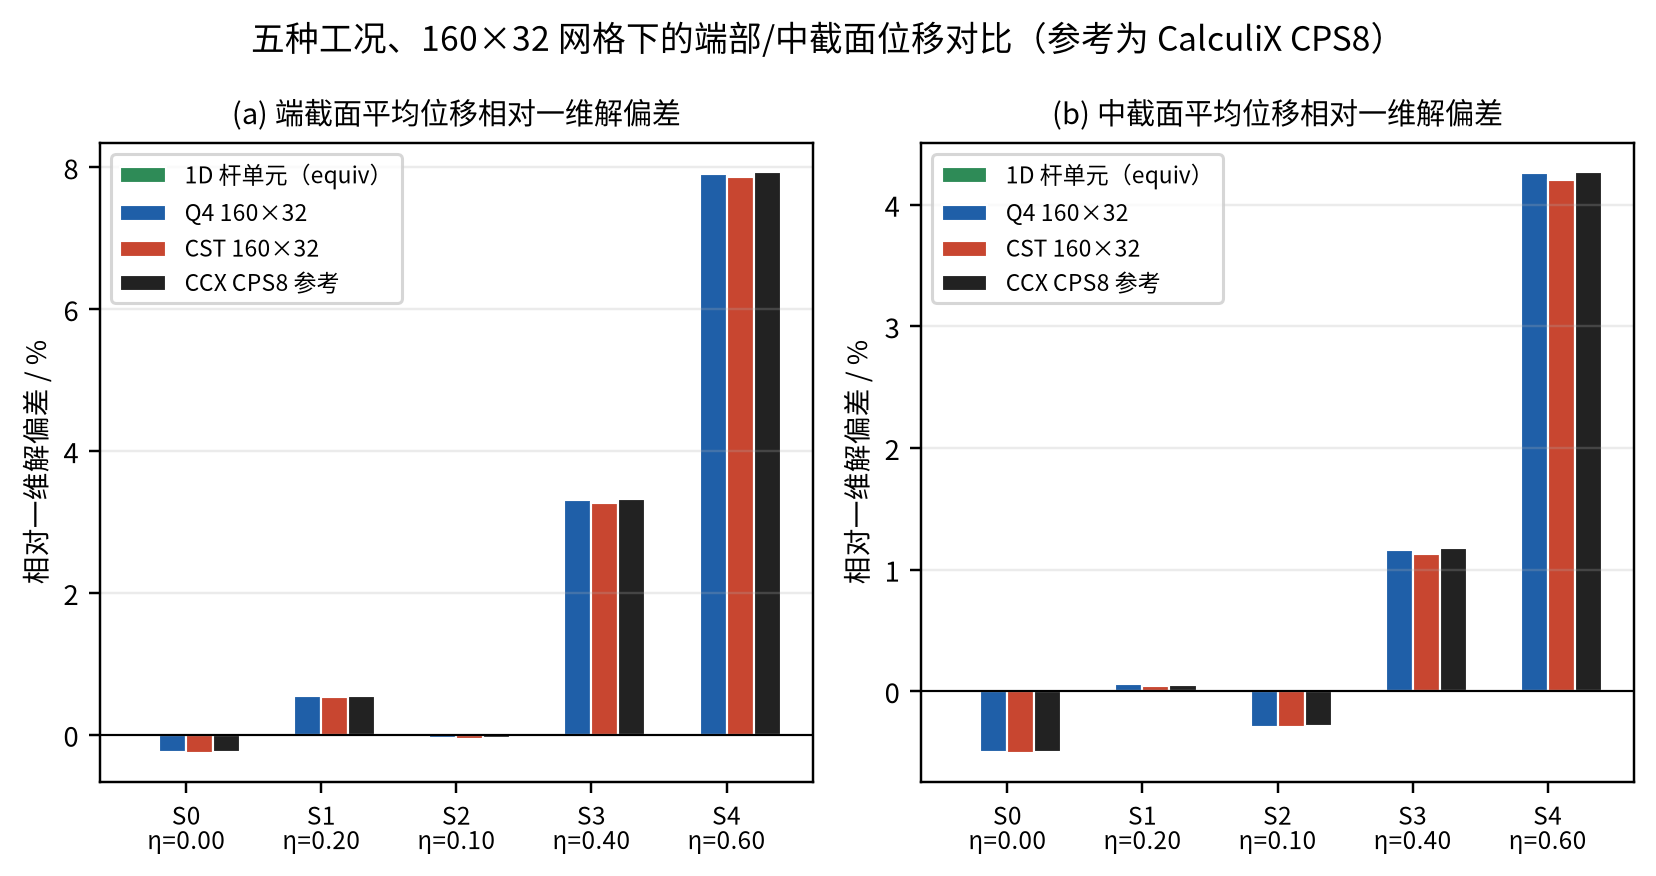
\includegraphics[width=\textwidth]{figures/fig02_displacement.png}
  \caption{五种工况在 $160\times32$ 网格下的端/中截面位移相对一维解的偏差。现象：S0、S1、S2 的偏差在 $1\%$ 以内，S3、S4 的偏差随 $\eta$ 迅速增大；Q4、CST 与 CCX 参考的柱高几乎重合。解读：小锥角下二维效应主要是端部边界层，一维名义解仍可用；大锥角下横向应力与楔形边缘效应成为一阶量，一维杆失效，而 Q4/CST 仍能跟踪参考。}
  \label{fig:displacement}
\end{figure}

值得注意的是，S0（$\beta=0$）的一维解与二维参考也有约 $0.25\%$ 的端部偏差、$0.50\%$ 的中截面偏差。这不是锥度效应，而是固定端全约束阻止泊松收缩造成的真实边界层；即便等截面杆，若关心端部位移，也应使用二维模型或至少做端部修正。

\subsection{名义应力沿轴曲线}

截面平均应力由平衡决定，任何满足平衡的离散解都应逼近 $\sigma_{\rm nom}=P/A(x)$；二维效应体现在应力沿截面的\textbf{非均匀分布}上。表~\ref{tab:stress-profile} 显示，S1 的内部截面平均值与 $P/A(x)$ 的差异在 $0.01\%$ 量级；表~\ref{tab:point-stress} 则显示，$y=0$ 处点应力在固定端附近比名义值高约 $1.8\%$，到中截面仍高约 $0.7\%$。图~\ref{fig:stress} 把这一差异画成沿轴曲线与截面分布。

\begin{table}[htbp]
  \centering
  \caption{S1 的截面平均轴向应力（kPa，$160\times32$）。内部站（$x/L=0.1$–$0.9$）的截面平均与名义值几乎重合。}
  \label{tab:stress-profile}
  \small
  \begin{tabular}{@{}S[table-format=1.1]S[table-format=2.2]S[table-format=2.2]S[table-format=2.2]S[table-format=2.2]@{}}
\toprule
{$x/L$} & {$\sigma_{\rm nom}$/kPa} & {CCX 截面平均/kPa} & {Q4 截面平均/kPa} & {CST 截面平均/kPa} \\
\midrule
0.1 & 45.45 & 45.45 & 45.45 & 45.45 \\
0.2 & 41.67 & 41.67 & 41.67 & 41.67 \\
0.3 & 38.46 & 38.46 & 38.46 & 38.46 \\
0.4 & 35.71 & 35.71 & 35.71 & 35.71 \\
0.5 & 33.33 & 33.33 & 33.33 & 33.33 \\
0.6 & 31.25 & 31.25 & 31.25 & 31.25 \\
0.7 & 29.41 & 29.41 & 29.41 & 29.41 \\
0.8 & 27.78 & 27.78 & 27.78 & 27.78 \\
0.9 & 26.32 & 26.32 & 26.32 & 26.32 \\
\bottomrule
\end{tabular}

\end{table}

\begin{table}[htbp]
  \centering
  \caption{S1 在 $y=0$ 处的轴向应力（kPa，$160\times32$）。参考值为 CalculiX CPS8 $240\times48$。}
  \label{tab:point-stress}
  \small
  \begin{tabular}{@{}S[table-format=1.1]S[table-format=2.2]S[table-format=2.2]S[table-format=2.2]@{}}
\toprule
{$x/L$} & {Q4 $\sigma_x(y=0)$/kPa} & {CST $\sigma_x(y=0)$/kPa} & {CCX $\sigma_x(y=0)$/kPa} \\
\midrule
0.1 & 46.28 & 46.27 & 46.30 \\
0.2 & 42.27 & 42.26 & 42.27 \\
0.5 & 33.55 & 33.55 & 33.55 \\
0.8 & 27.36 & 27.37 & 27.37 \\
0.9 & 25.60 & 25.61 & 25.61 \\
\bottomrule
\end{tabular}

\end{table}

\begin{figure}[htbp]
  \centering
  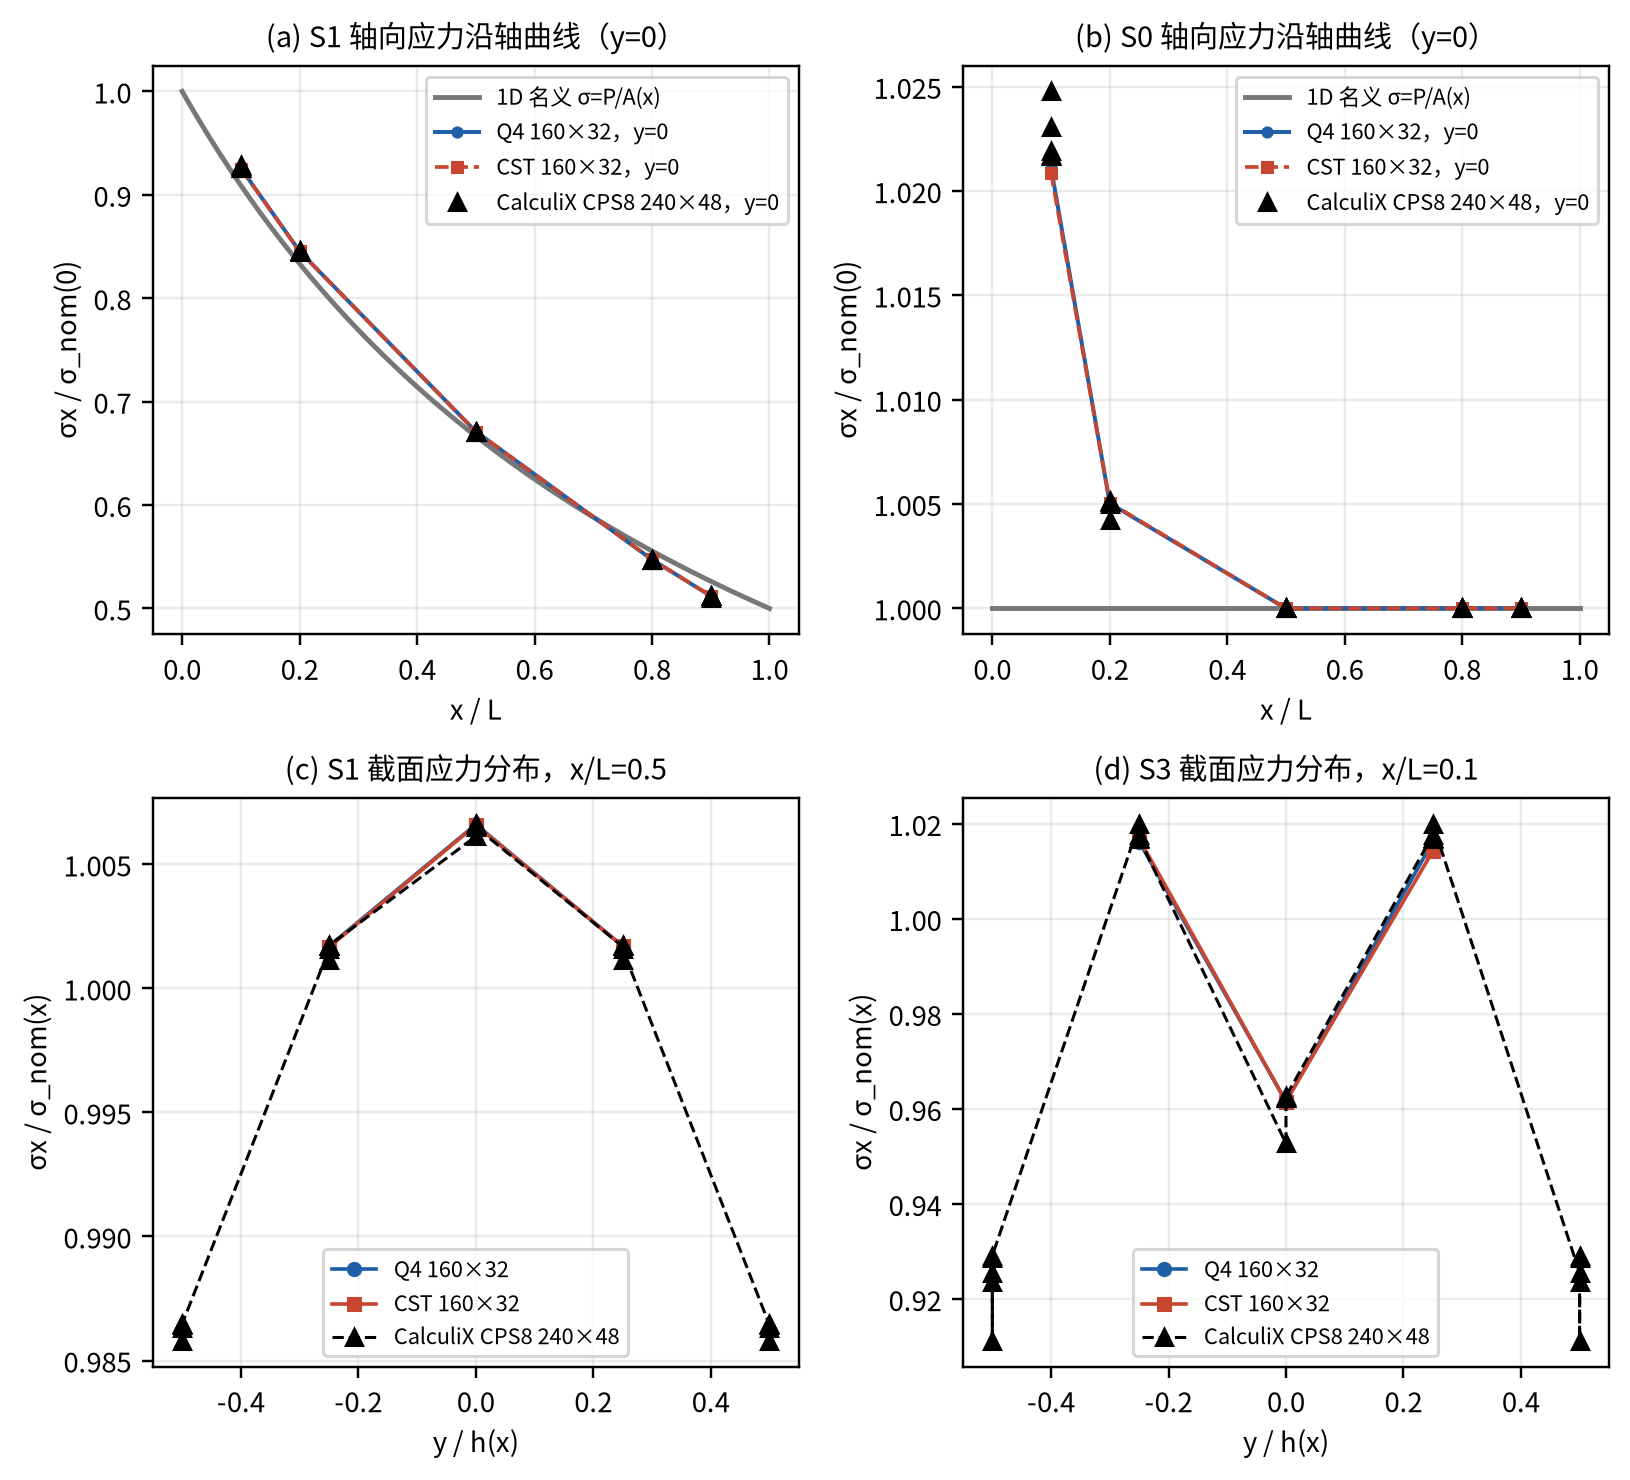
\includegraphics[width=\textwidth]{figures/fig03_stress_profile.png}
  \caption{轴向应力沿轴曲线与截面应力分布。现象：S1 的 $\sigma_x$ 沿轴由约 $50\,\mathrm{kPa}$ 平滑降至 $25\,\mathrm{kPa}$；Q4、CST 与 CCX 在 $y=0$ 处几乎重合，但 CST 在截面边缘略低；S3 的近固定端截面呈明显的“中间低、两侧高”分布。解读：截面平均应力由平衡控制，因而各方法一致；点应力差异反映二维楔形效应与端部约束，S3/S4 的截面非均匀性显著增强，正是一维判据失效的微观表现。}
  \label{fig:stress}
\end{figure}

\subsection{应力与位移收敛}

Q4、CST 的应力和位移误差均随网格单调下降；Q4 的应力阶略高，CST 的局部应力误差更大但同样稳定收敛。应力误差与拟合阶列于 表~\ref{tab:conv}，双对数曲线见图~\ref{fig:conv}。Q4 的探针应力误差为 $0.015\%$–$0.042\%$，CST 为 $0.020\%$–$0.146\%$；Q4 的位移观测阶约 $1.7$–$2.5$（S1 端部因误差已接近参考精度呈超收敛），CST 约 $1.5$–$2.4$。

\begin{table}[htbp]
  \centering
  \caption{应力误差与观测收敛阶。$e$ 为 $160\times32$ 的相对误差（\%），$p$ 由 $40\times8$、$80\times16$、$160\times32$ 三点拟合。CST 的梯度保真误差未定义，以“--”表示。}
  \label{tab:conv}
  \footnotesize
  \setlength{\tabcolsep}{3.5pt}
  \begin{tabular}{@{}llS[table-format=1.4]S[table-format=1.2]S[table-format=1.5]S[table-format=1.2]S[table-format=1.3]S[table-format=1.2]@{}}
\toprule
工况 & 方法 & {$e_{\sigma,\rm probe}$/\%} & {$p_{\rm probe}$} & {$e_{\sigma,\rm profile}$/\%} & {$p_{\rm profile}$} & {$e_{\rm grad}$/\%} & {$p_{\rm grad}$} \\
\midrule
S0 & Q4 & 0.0183 & 1.05 & 0.00007 & 0.00 & \multicolumn{1}{c}{--} & \multicolumn{1}{c}{--} \\
S0 & CST & 0.0258 & 1.32 & 0.00007 & -0.00 & \multicolumn{1}{c}{--} & \multicolumn{1}{c}{--} \\
S1 & Q4 & 0.0197 & 1.58 & 0.00040 & 2.23 & 0.633 & 1.27 \\
S1 & CST & 0.0372 & 1.67 & 0.00039 & 2.27 & \multicolumn{1}{c}{--} & \multicolumn{1}{c}{--} \\
S2 & Q4 & 0.0147 & 0.83 & 0.00025 & 2.55 & 0.347 & 1.65 \\
S2 & CST & 0.0200 & 1.21 & 0.00020 & 2.63 & \multicolumn{1}{c}{--} & \multicolumn{1}{c}{--} \\
S3 & Q4 & 0.0417 & 1.85 & 0.00127 & 1.46 & 0.945 & 1.04 \\
S3 & CST & 0.1019 & 1.60 & 0.00127 & 1.56 & \multicolumn{1}{c}{--} & \multicolumn{1}{c}{--} \\
S4 & Q4 & 0.0395 & 2.04 & 0.00211 & 1.88 & 0.899 & 1.25 \\
S4 & CST & 0.1458 & 1.62 & 0.00203 & 1.97 & \multicolumn{1}{c}{--} & \multicolumn{1}{c}{--} \\
\bottomrule
\end{tabular}

\end{table}

\begin{figure}[htbp]
  \centering
  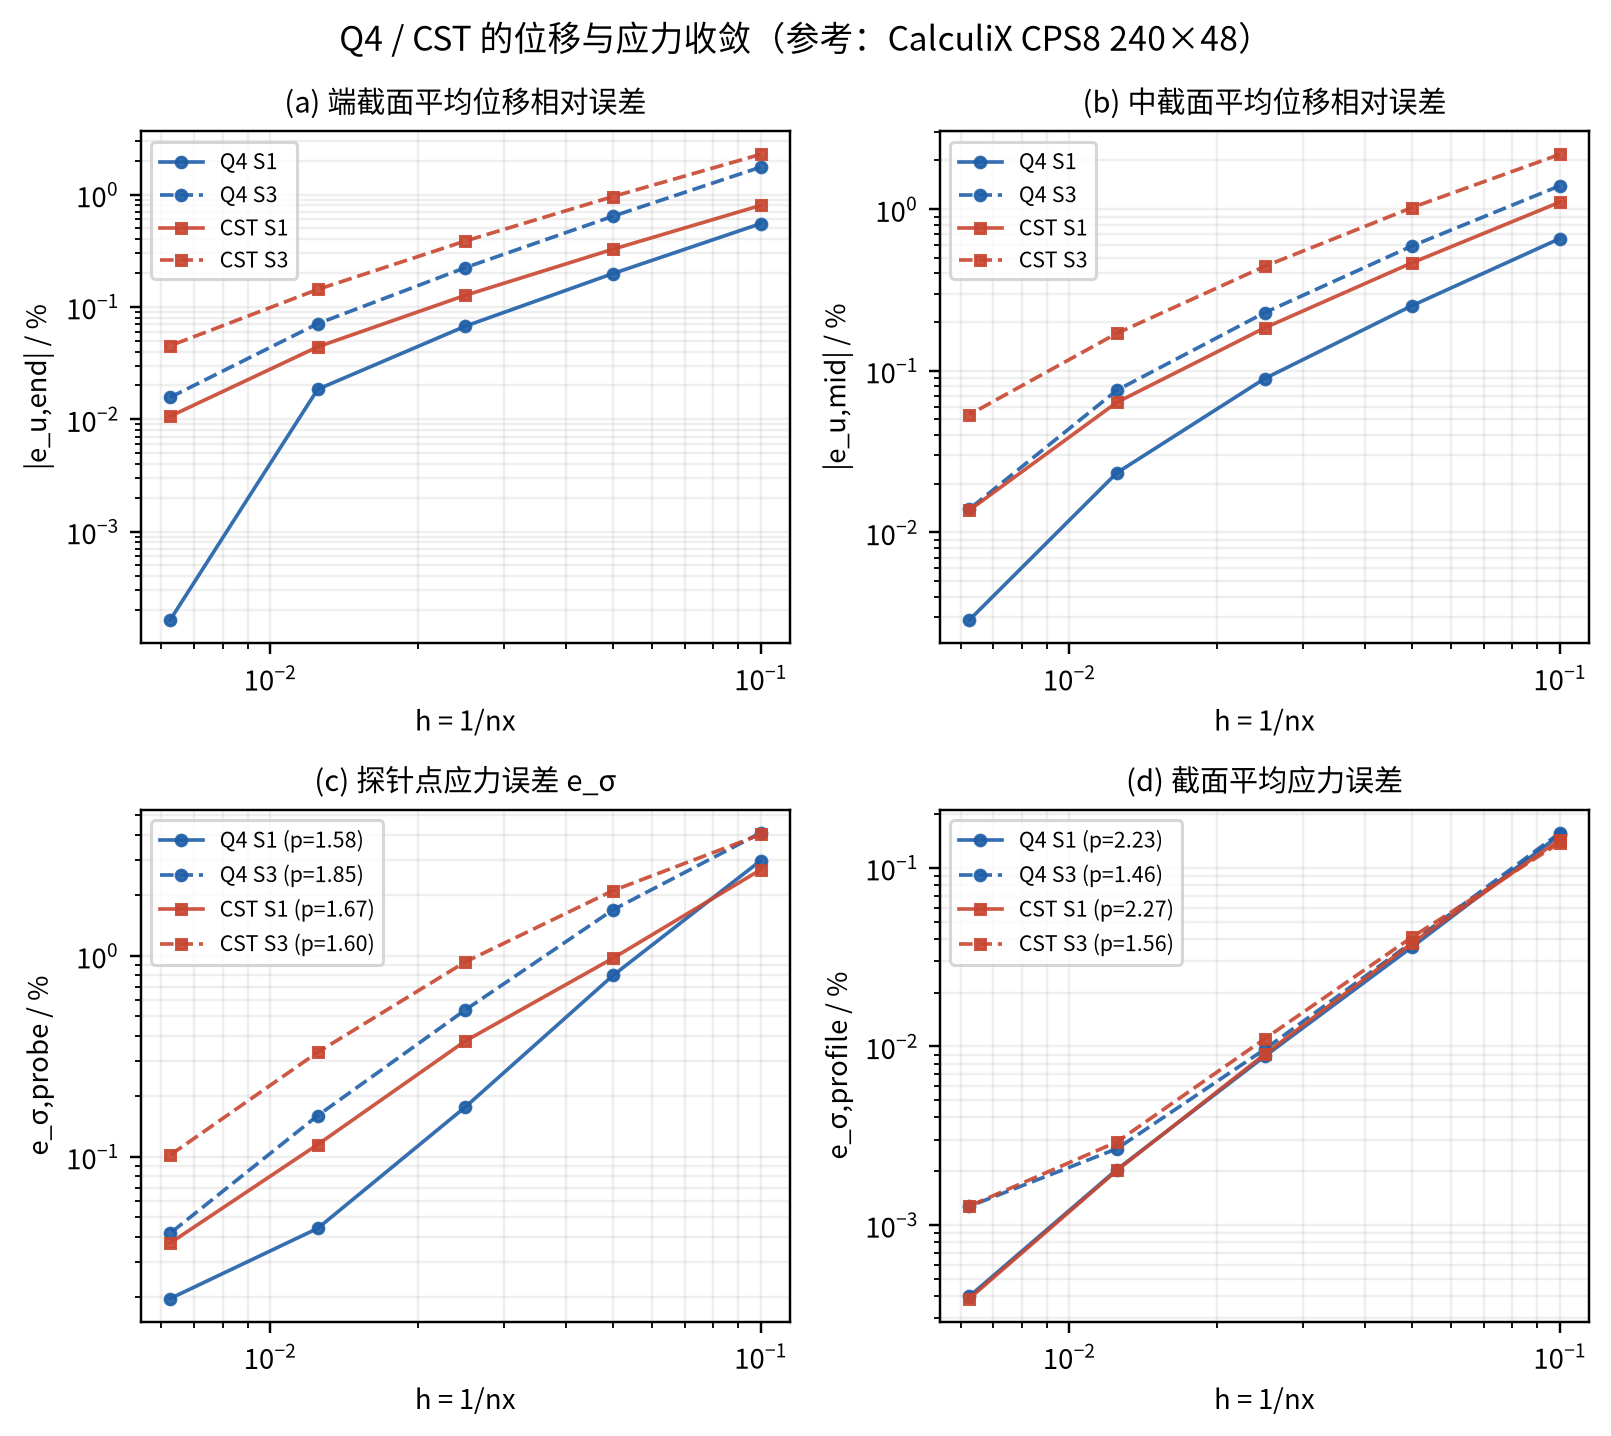
\includegraphics[width=\textwidth]{figures/fig04_convergence.png}
  \caption{Q4/CST 的位移与应力误差随 $h=1/n_x$ 的变化。现象：四个子图的误差均随 $h$ 减小而下降，应力子图的拟合阶集中在 $1.6$–$2.3$；位移子图在细网格端趋于平缓。解读：应力采用点值探针，误差量级更小且阶数稳定；位移误差在细网格受参考解精度与端部边界层限制，拟合阶出现分散，不宜单独作为方法精度判据。}
  \label{fig:conv}
\end{figure}

\subsection{梯度保真与剪切能比}

Q4 对截面平均应力梯度的复现误差为 $0.35\%$–$0.95\%$，随网格以约 $1.0$–$1.7$ 阶下降；剪切能比 $R_s$ 随 $\eta$ 单调增大，定量印证了一维判据。这组结果列于 表~\ref{tab:grad}，并绘于 图~\ref{fig:grad}。

\begin{table}[htbp]
  \centering
  \caption{Q4 的梯度保真误差 $e_{\rm grad}$、拟合阶 $p_{\rm grad}$ 与剪切能比 $R_s$（$160\times32$）。S0 的名义梯度为零，$e_{\rm grad}$ 无定义。}
  \label{tab:grad}
  \small
  \begin{tabular}{@{}lS[table-format=1.2]S[table-format=1.3]S[table-format=1.2]S[table-format=1.3]@{}}
\toprule
工况 & {$\eta$} & {$e_{\rm grad}$/\%} & {$p_{\rm grad}$} & {$R_s$/\%} \\
\midrule
S0 & 0.00 & \multicolumn{1}{c}{--} & \multicolumn{1}{c}{--} & 0.177 \\
S1 & 0.20 & 0.633 & 1.27 & 0.643 \\
S2 & 0.10 & 0.347 & 1.65 & 0.215 \\
S3 & 0.40 & 0.945 & 1.04 & 2.393 \\
S4 & 0.60 & 0.899 & 1.25 & 4.870 \\
\bottomrule
\end{tabular}

\end{table}

\begin{figure}[htbp]
  \centering
  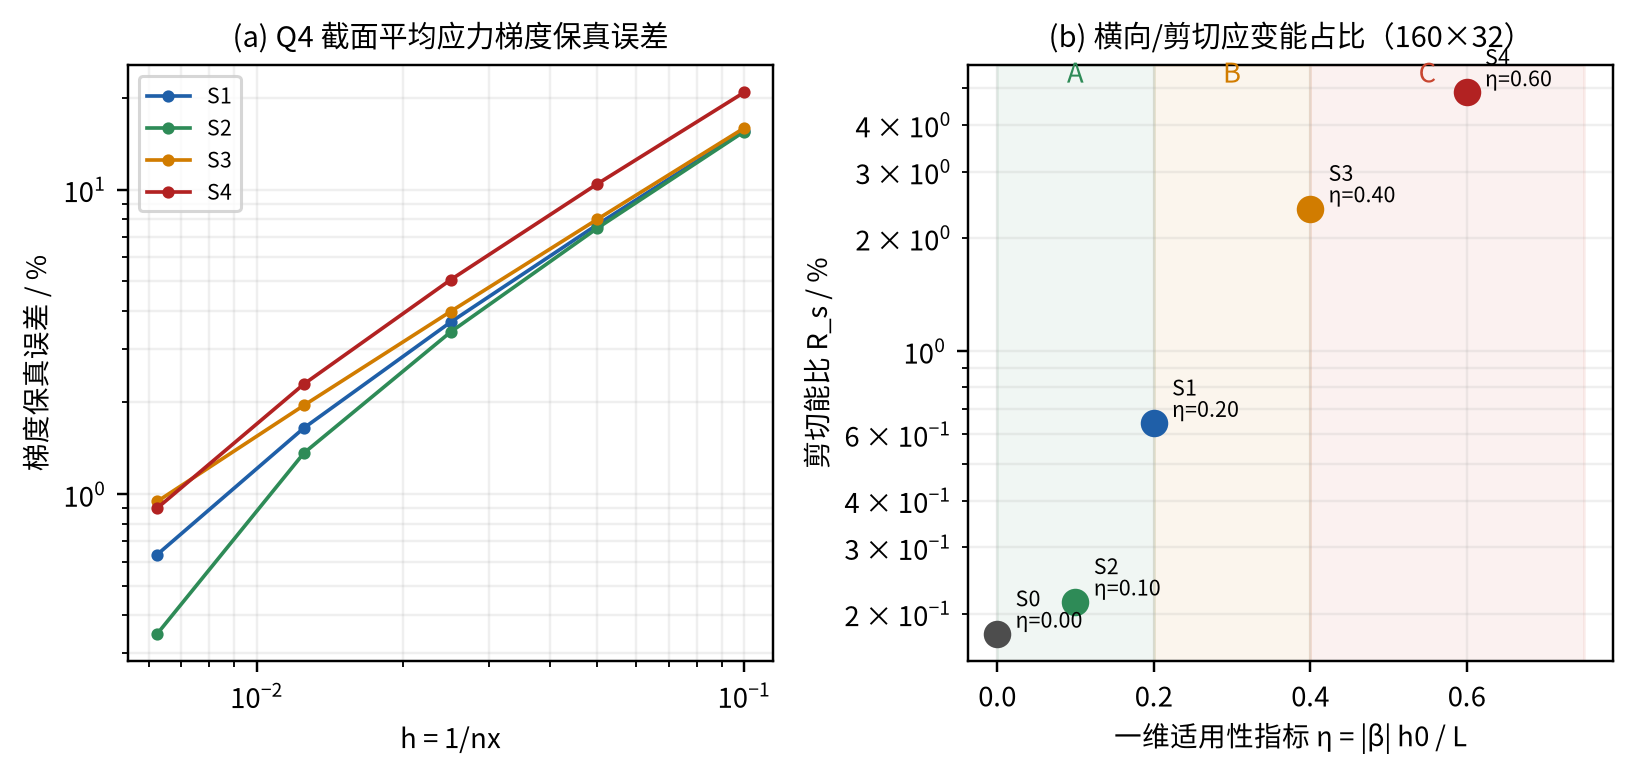
\includegraphics[width=\textwidth]{figures/fig05_gradient_shear.png}
  \caption{梯度保真误差与剪切能比。现象：$e_{\rm grad}$ 随 $h$ 下降，$R_s$ 随 $\eta$ 从 S0 的 $0.18\%$ 增至 S4 的 $4.87\%$。解读：前者说明 Q4 的线性应力场能稳定复现截面平均应力的梯度；后者说明大锥角下横向/剪切能量占比显著上升，一维单轴假设不再成立。}
  \label{fig:grad}
\end{figure}

\subsection{CST 对角线离散度与面积加权恢复}

CST 的全局量对剖分方向不敏感，但局部应力敏感：端/中位移与截面平均应力的对角线离散度为 $10^{-11}\%$ 量级，而单元应力与恢复后节点应力的局部离散度在 $160\times32$ 下为 $0.24\%$–$1.07\%$ 与 $0.31\%$–$2.47\%$。具体对比见表~\ref{tab:diag} 与图~\ref{fig:diag}。

\begin{table}[htbp]
  \centering
  \caption{CST 对角线离散度与截面内离散系数（$160\times32$）。$D_u$、$D_{\sigma,\rm ax}$ 为镜像不变量，理论上应为零；$D_{\sigma,\rm el}$、$D_{\sigma,\rm node}$ 为局部敏感度。}
  \label{tab:diag}
  \footnotesize
  \setlength{\tabcolsep}{3pt}
  \begin{tabular}{@{}lS[table-format=1.2e-2]S[table-format=1.2e-2]S[table-format=1.3]S[table-format=1.3]S[table-format=2.2]S[table-format=2.2]@{}}
\toprule
工况 & {$D_u$/\%} & {$D_{\sigma,\rm ax}$/\%} & {$D_{\sigma,\rm el}$/\%} & {$D_{\sigma,\rm node}$/\%} & {$CV_{\rm raw}$/\%} & {$CV_{\rm rec}$/\%} \\
\midrule
S0 & 6.26e-12 & 1.63e-11 & 0.293 & 0.508 & 2.12 & 2.22 \\
S1 & 1.52e-11 & 1.72e-11 & 0.527 & 1.025 & 3.20 & 3.38 \\
S2 & 2.04e-11 & 2.11e-11 & 0.235 & 0.308 & 2.46 & 2.56 \\
S3 & 7.65e-12 & 1.02e-11 & 0.570 & 1.659 & 6.61 & 7.09 \\
S4 & 6.88e-12 & 8.13e-12 & 1.069 & 2.466 & 9.54 & 10.06 \\
\bottomrule
\end{tabular}

\end{table}

\begin{figure}[htbp]
  \centering
  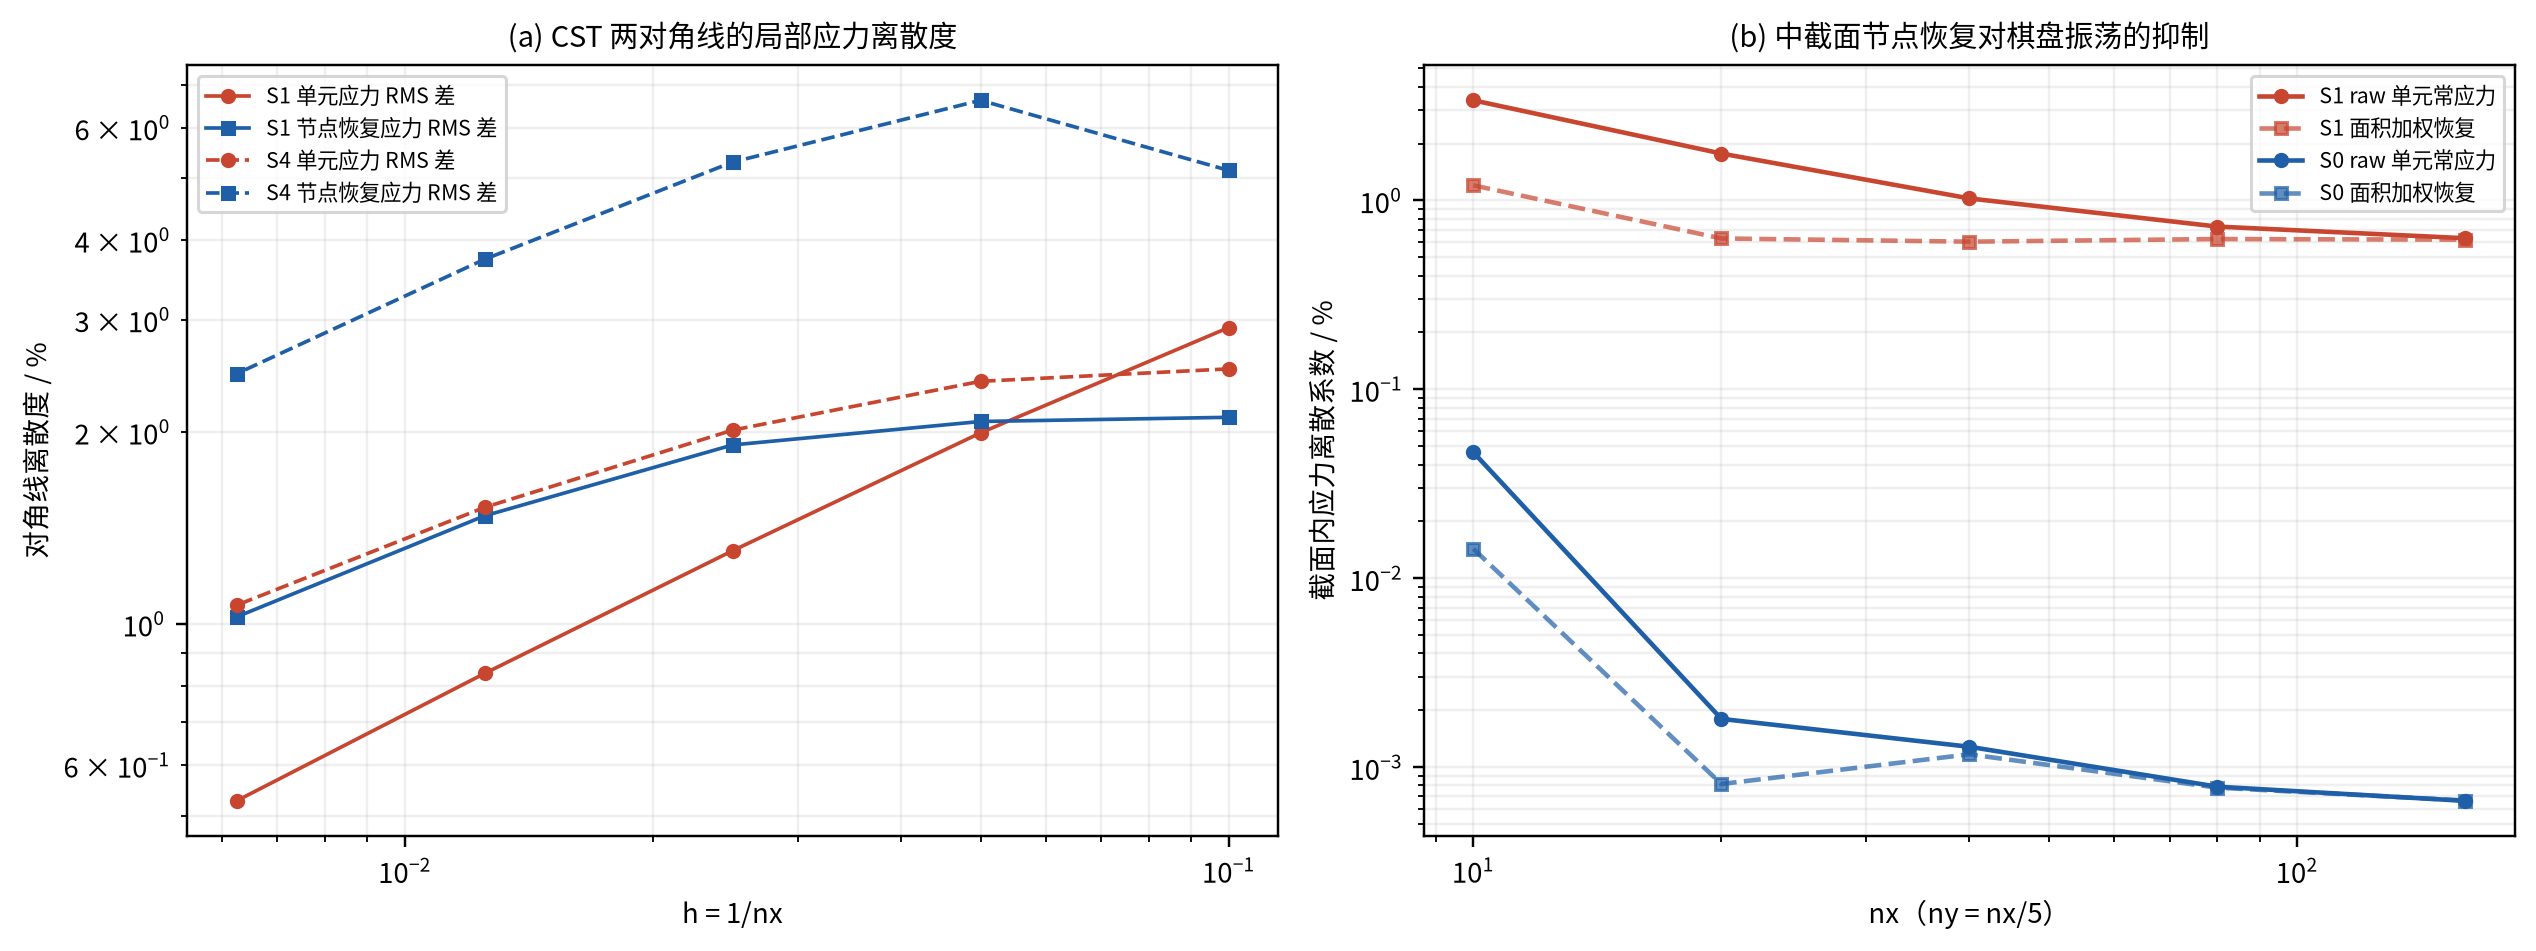
\includegraphics[width=\textwidth]{figures/fig06_cst_diagonal.png}
  \caption{CST 对角线离散度与节点恢复。现象：局部应力离散度随网格下降，S4 的离散度显著高于 S1；面积加权恢复在粗网格上降低了截面内 $CV$，细网格上与 raw 接近。解读：对称工况下剖分方向只影响局部场，不影响全局位移；面积加权恢复主要抑制粗网格的棋盘振荡，不能替代网格加密。}
  \label{fig:diag}
\end{figure}

\subsection{一维杆适用性判据与可信度标签}

一维杆的等效刚度若采用柔度积分，节点位移与解析解一致到 $10^{-13}$ 且与网格无关；用平均面积刚度则会在粗网格下高估刚度、低估端位移。各工况的标签与后验偏差列于 表~\ref{tab:bar}，判据区间见图~\ref{fig:bar}。S0/S1/S2 判为 A，S3 为 B，S4 为 C；端部偏差依次为 $+0.25\%$、$-0.55\%$、$+0.05\%$、$-3.21\%$、$-7.36\%$，与标签分级一致。

\begin{table}[htbp]
  \centering
  \caption{一维杆可信度标签与后验校核。偏差定义为 $(u_{\rm bar}-u_{\rm ccx})/u_{\rm ccx}$（\%）。}
  \label{tab:bar}
  \small
  \begin{tabular}{@{}lS[table-format=1.2]S[table-format=2.1]cS[table-format=+1.2]S[table-format=+1.2]@{}}
\toprule
工况 & {$\eta$} & {锥角/$^\circ$} & 标签 & {端部偏差/\%} & {中截面偏差/\%} \\
\midrule
S0 & 0.00 & 0.0 & A & +0.25 & +0.50 \\
S1 & 0.20 & 11.3 & A & -0.55 & -0.05 \\
S2 & 0.10 & 5.7 & A & +0.05 & +0.29 \\
S3 & 0.40 & 21.8 & B & -3.21 & -1.16 \\
S4 & 0.60 & 31.0 & C & -7.36 & -4.10 \\
\bottomrule
\end{tabular}

\end{table}

\begin{figure}[htbp]
  \centering
  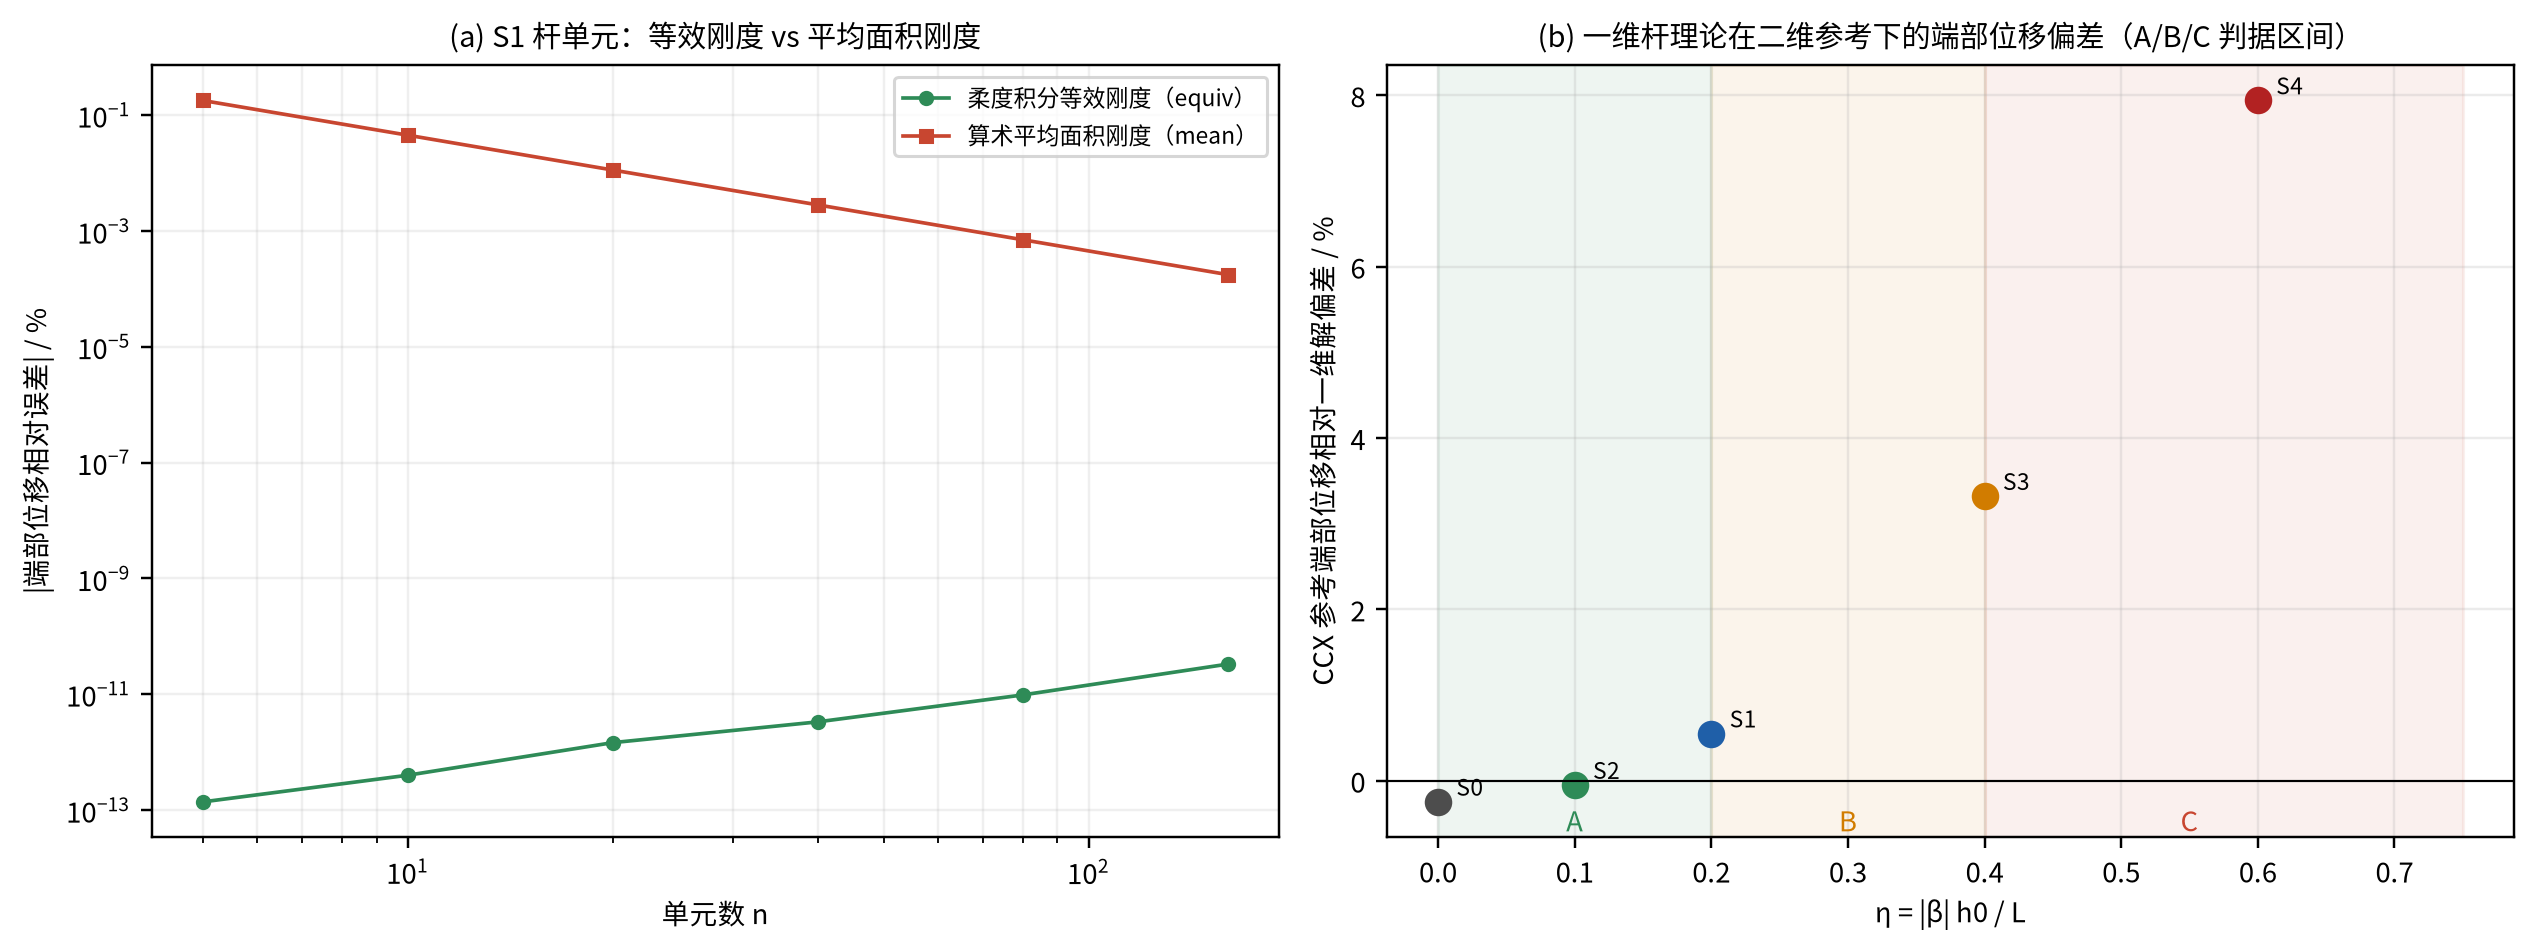
\includegraphics[width=\textwidth]{figures/fig07_bar.png}
  \caption{杆单元刚度对比与一维判据。现象：柔度积分等效刚度的端位移误差保持在 $10^{-11}\%$ 以下的舍入量级；平均面积刚度误差按 $O(h^2)$ 下降；二维参考下的一维端部偏差随 $\eta$ 从 $+0.25\%$ 变到 $-7.36\%$。解读：节点精确性只说明 1D 方程解对了，不能消除 1D 模型本身的模型误差；A/B/C 分级应结合 $\eta$ 与后验偏差，而不能只看网格收敛。}
  \label{fig:bar}
\end{figure}

\subsection{CalculiX 锚点与端载敏感性}
\label{sec:anchor}

CalculiX 的 CPS8 $240\times48$ 参考与自研 Q4/CST 高度一致：Q4 的端位移偏差为 $0.000$–$0.025\%$，CST 为 $0.001$–$0.075\%$（表~\ref{tab:anchor}、图~\ref{fig:anchor}）。同网格 CPS4 与 Q4 的端位移差最大 $0.049\%$，说明单元公式、组装、边界与载荷实现正确。端载从一致面力改为等分节点力时，$u_{\rm end}$ 变化不超过 $0.281\%$，但加载端局部节点应力可差 $1\%$–$8\%$（表~\ref{tab:load}），因此点值应力对比必须统一口径。

\begin{table}[htbp]
  \centering
  \caption{CalculiX CPS8 $240\times48$ 参考与自研方法的端位移对照（Q4/CST 取 $160\times32$）。}
  \label{tab:anchor}
  \small
  \begin{tabular}{@{}lS[table-format=1.4e-2]S[table-format=1.4e-2]S[table-format=+1.3]S[table-format=1.4e-2]S[table-format=+1.3]@{}}
\toprule
工况 & {CPS8 $u_{\rm end}$/m} & {Q4 $u_{\rm end}$/m} & {Q4 偏差/\%} & {CST $u_{\rm end}$/m} & {CST 偏差/\%} \\
\midrule
S0 & 2.4938e-07 & 2.4938e-07 & -0.000 & 2.4937e-07 & -0.005 \\
S1 & 1.7424e-07 & 1.7424e-07 & -0.000 & 1.7422e-07 & -0.011 \\
S2 & 3.4639e-07 & 3.4640e-07 & 0.002 & 3.4639e-07 & -0.001 \\
S3 & 8.9520e-08 & 8.9506e-08 & -0.016 & 8.9480e-08 & -0.045 \\
S4 & 9.8819e-08 & 9.8794e-08 & -0.025 & 9.8745e-08 & -0.075 \\
\bottomrule
\end{tabular}

\end{table}

\begin{table}[htbp]
  \centering
  \caption{端载离散口径敏感性：一致面力与等分节点力的绝对差（\%）。}
  \label{tab:load}
  \small
  \begin{tabular}{@{}lS[table-format=1.3]S[table-format=1.3]@{}}
\toprule
工况 & {$\Delta u_{\rm end}$/\%} & {$\Delta u_{\rm mid}$/\%} \\
\midrule
S0 & 0.016 & 0.000 \\
S1 & 0.062 & 0.000 \\
S2 & 0.001 & 0.000 \\
S3 & 0.207 & 0.015 \\
S4 & 0.281 & 0.017 \\
\bottomrule
\end{tabular}

\end{table}

\begin{figure}[htbp]
  \centering
  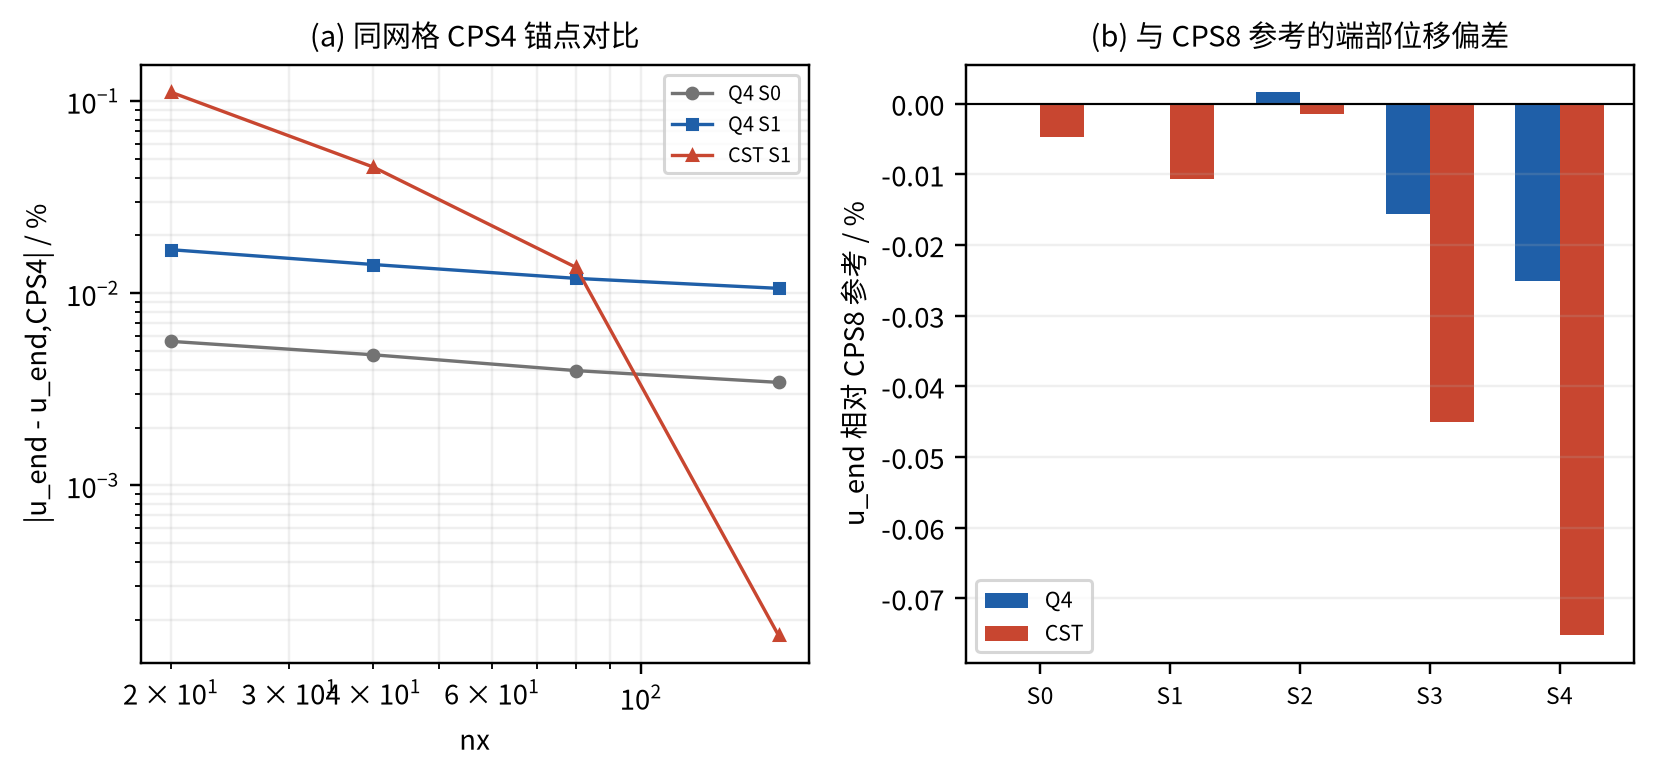
\includegraphics[width=\textwidth]{figures/fig08_anchor.png}
  \caption{与 CalculiX 的锚点对比。现象：同网格 Q4 与 CPS4 的差在 $10^{-2}\%$ 量级并随网格减小；CST 在粗网格的差明显更大，$160\times32$ 时降到 $10^{-3}\%$ 以下；自研 Q4/CST 与 CPS8 参考的端位移差均小于 $0.08\%$。解读：自研单元与 CalculiX 的实现一致，剩余差异来自 CalculiX 将平面应力单元展开为三维单元的厚度积分细节；CST 的粗网格差异主要来自常应变假设。}
  \label{fig:anchor}
\end{figure}

\subsection{FEniCS 可选本构校核}
\label{sec:fenics}

FEniCS/dolfinx 0.11 以 P2 三角形、$80\times16$ 网格、一致面力对 S0/S1 做独立校核：S0 的 $u_{\rm end}=2.493808\times10^{-7}\,\mathrm{m}$，与一维解的偏差来自固定端泊松约束；S1 的 $u_{\rm end}=1.742433\times10^{-7}\,\mathrm{m}$，与 CCX $240\times48$ 参考仅差 $+0.0029\%$。两个独立第三方求解器互证了锚点参考值（表~\ref{tab:fenics}）。

\begin{table}[htbp]
  \centering
  \caption{FEniCS 本构/位移校核（P2 三角形，$80\times16$）。}
  \label{tab:fenics}
  \small
  \begin{tabular}{@{}lS[table-format=1.4e-2]S[table-format=1.4e-2]S[table-format=+1.3]S[table-format=5.2]@{}}
\toprule
工况 & {FEniCS $u_{\rm end}$/m} & {1D $u_{\rm end}$/m} & {偏差/\%} & {$\sigma_{\rm mid}$/Pa} \\
\midrule
S0 & 2.4938e-07 & 2.5000e-07 & -0.248 & 50000.00 \\
S1 & 1.7424e-07 & 1.7329e-07 & 0.552 & 33445.12 \\
\bottomrule
\end{tabular}

\end{table}

\subsection{变形与应力云图}

S1 在 $40\times8$ 网格下的变形与 $\sigma_x$ 云图（图~\ref{fig:deformed}）显示：变形放大 $2.5\times10^5$ 后，楔形段整体伸长，$\sigma_x$ 从固定端到自由端逐渐降低，与 $P/A(x)$ 的趋势一致。

\begin{figure}[htbp]
  \centering
  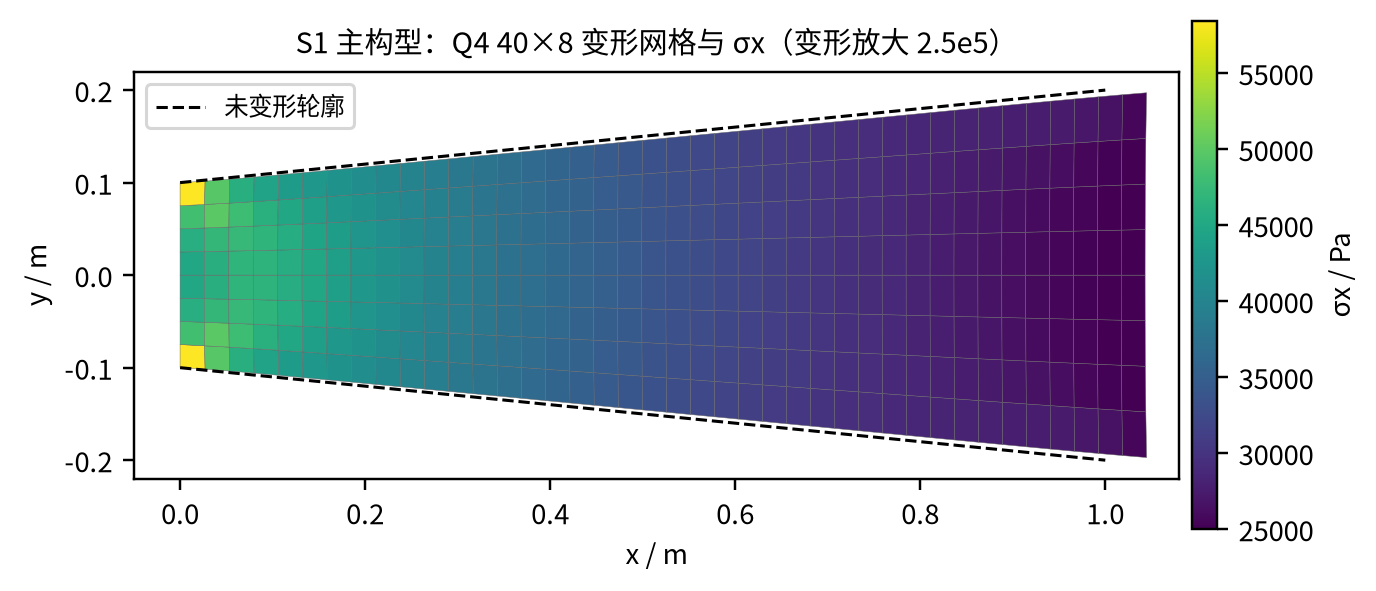
\includegraphics[width=0.86\textwidth]{figures/fig09_deformed.png}
  \caption{S1 的变形网格与 $\sigma_x$ 云图（Q4，$40\times8$，变形放大 $2.5\times10^5$）。现象：楔形段整体伸长，固定端附近出现明显的应力集中，自由端应力最低。解读：这正是二维模型相对一维杆的附加信息——一维杆只能给出截面平均值，无法显示端部与边缘的局部应力梯度。}
  \label{fig:deformed}
\end{figure}